%%%%%%%%%%%%%%%%%%%%%%%%%%%%%%%%%%%%%%%%%%%%%%%%%%%%%%%%%%%%%%%%%%%%%%%%%%%%%%%%
%2345678901234567890123456789012345678901234567890123456789012345678901234567890
%        1         2         3         4         5         6         7         8

\documentclass[letterpaper, 10 pt, conference]{ieeeconf}  % Comment this line out if you need a4paper

%\documentclass[a4paper, 10pt, conference]{ieeeconf}      % Use this line for a4 paper

\IEEEoverridecommandlockouts                              % This command is only needed if 
                                                          % you want to use the \thanks command

\overrideIEEEmargins                                      % Needed to meet printer requirements.

%In case you encounter the following error:
%Error 1010 The PDF file may be corrupt (unable to open PDF file) OR
%Error 1000 An error occurred while parsing a contents stream. Unable to analyze the PDF file.
%This is a known problem with pdfLaTeX conversion filter. The file cannot be opened with acrobat reader
%Please use one of the alternatives below to circumvent this error by uncommenting one or the other
%\pdfobjcompresslevel=0
%\pdfminorversion=4

% See the \addtolength command later in the file to balance the column lengths
% on the last page of the document

% The following packages can be found on http:\\www.ctan.org
%\usepackage{graphics} % for pdf, bitmapped graphics files
%\usepackage{epsfig} % for postscript graphics files
%\usepackage{mathptmx} % assumes new font selection scheme installed
%\usepackage{times} % assumes new font selection scheme installed
%\usepackage{amsmath} % assumes amsmath package installed
%\usepackage{amssymb}  % assumes amsmath package installed
\usepackage{graphicx}
\usepackage{epstopdf}
\usepackage{amsmath}
\usepackage{amssymb}
\usepackage{subfigure}
\usepackage{multirow}
\usepackage{pbox}
\usepackage{algorithm}
\usepackage{algorithmic}
%\usepackage{algpseudocode}
\usepackage{bm}
\usepackage{url}
\newcommand\NB[1]{$\spadesuit$\footnote{NB: #1}}
\newcommand\RP[1]{$\clubsuit$\footnote{RP: #1}}

\newcommand{\R}{\mathbb{R}}
\newcommand{\Z}{\mathbb{Z}}
\newcommand{\D}{\mathbb{D}}
\newcommand{\N}{\mathbb{N}}

\newtheorem{problem}{Problem}
\newtheorem{lemma}{Lemma}

\DeclareMathOperator*{\argmin}{arg\,min}
\DeclareMathOperator*{\argmax}{arg\,max}

\begin{document}

\title{\LARGE \bf
Teleop Command/Imitation Learning/Regression (in progress)
}


\author{Rahul Peddi and Nicola Bezzo%
\thanks{Rahul Peddi and Nicola Bezzo are with the Department of Systems and Information Engineering and the Charles L. Brown Department of Electrical and Computer Engineering, University of Virginia, Charlottesville, VA 22904, USA. Email: {\tt \{rp3cy, nb6be\}@virginia.edu}}}



\maketitle
\thispagestyle{empty}
\pagestyle{empty}


%%%%%%%%%%%%%%%%%%%%%%%%%%%%%%%%%%%%%%%%%%%%%%%%%%%%%%%%%%%%%%%%%%%%%%%%%%%%%%%%
\begin{abstract}


\end{abstract}


%%%%%%%%%%%%%%%%%%%%%%%%%%%%%%%%%%%%%%%%%%%%%%%%%%%%%%%%%%%%%%%%%%%%%%%%%%%%%%%%
\section{Introduction}
Unmanned Aerial Vehicles have become more widespread for both civilian and military applications in the recent years. T
\section{Related Work}


\section{Problem Formulation}
In this work, we are interested in finding a policy that enables autonomous UAV navigation over a user-defined trajectory.

Formally, the problem we investigate in this work can be stated as:

%\NB{problem is still not good. What is the problem that you are trying to solve? It's not processing and analyzing data!}
\textbf{Problem 1: \textit{Demonstration-based autonomous control generation}}: A UAV has the objective to visit a set of $n$ goals, $\mathbf{g}\in\mathbb{R}^{n}$, at a set of $n$ target times, $\mathbf{t} \in\mathbb{R}^{n}$. Given $m$ human-piloted flight demonstrations, the aim is to find a policy that enables autonomous flight to generate and track a trajectory $\mathbf{p_r}(t),~ t \in [0,T]$ that visits the target goals $\mathbf{g}_i$ at the respective target times, $\mathbf{t}_i$, such that the following liveness and promptness requirements are met:
\begin{enumerate}
    \item  Liveness: The UAV should always stay within a certain distance of the generated trajectory:
    \begin{equation}
        ||\mathbf{p}(t)-\mathbf{p_r}(t)|| \leq \delta_d,~\forall t \in [0,T]
    \end{equation}
    where $\mathbf{p_r}(t)$ is the reference position at time $t$, where $T$ represents an overall time horizon for the trajectory, and $\delta_d$ is a threshold for allowable deviation.
    \item  Promptness: The UAV should always reach the target locations within a certain threshold of the target time for that goal:
    \begin{align}
        \tau = t\in[0,T]|\mathbf{p}(t)-\mathbf{g}_i \leq \delta_d \nonumber \\
        |\tau- \mathbf{t}_i| \leq \delta_t,~i=1,\ldots,n
    \end{align}
    where $\tau$ is a time at which the liveness condition is met for a specific goal and $\delta_t$ is the allowable deviation in time from the target.
\end{enumerate}


\section{System Dynamics}
The type of UAV in question is modeled using a $12^{\text{th}}$ order state vector:
\begin{equation}
    \mathbf{q} = 
    \begin{bmatrix}
    \mathbf{p}_q^\intercal & \phi & \theta & \psi & v_x & v_y & v_z & \omega_x & \omega_y & \omega_z
    \end{bmatrix}^\intercal \nonumber
\end{equation} %\NB{what's the point of this section? What are you trying to demonstrate here?} 
where $\bm{p}_q=[x \; y \; z]^{\mathsf{T}}$ is the world frame position, $v_{x}$, $v_{y}$ and $v_z$ are the world frame velocities, $\phi$, $\theta$ and $\psi$ are the roll, pitch and yaw Euler angles and $\omega_{x}$, $\omega_{y}$ and $\omega_{z}$ are the body frame angular velocities.

The dynamics of the vehicle are then described as follows:
\begin{equation}
	\begin{aligned}
	%\begin{bmatrix}\dot{x} \\ \dot{y} \\ \dot{z} \end{bmatrix} &= \begin{bmatrix}v_x \\ v_y \\ v_z\end{bmatrix}\\
	\dot{\bm{p}_q}^{\mathsf{T}} &= \begin{bmatrix}v_x & v_y & v_z\end{bmatrix}\\
	\begin{bmatrix}\dot{v}_x \\ \dot{v}_y \\ \dot{v}_z\end{bmatrix} &= \begin{bmatrix}0 \\ 0 \\ -g \end{bmatrix} + \frac{1}{m} \begin{bmatrix}\cos\phi \cos\psi \sin\theta + \sin\phi \sin\psi \\ \cos\phi \sin\theta \sin\psi - \cos\psi \sin\phi \\ \cos\theta \cos\phi \end{bmatrix} u_1\\
	%\end{align*}
	%\begin{align*}
	\begin{bmatrix}\dot{\phi} \\ \dot{\theta} \\ \dot{\psi}\end{bmatrix} &= \begin{bmatrix}1 & \sin\phi \tan\theta & \cos\phi \tan\theta\\ 0 & \cos\phi & -\sin\phi \\ 0 & \sin\phi \sec\theta & \cos\phi \sec\theta \end{bmatrix} \begin{bmatrix}\omega_{x} \\ \omega_{y} \\ \omega_{z} \end{bmatrix}\\
	\begin{bmatrix}\dot{\omega}_{x} \\ \dot{\omega}_{y} \\ \dot{\omega}_{z}\end{bmatrix} &= \begin{bmatrix}\frac{I_{yy} - I_{zz}}{I_{xx}} \omega_{y}\omega_{z}\\ \frac{I_{zz} - I_{xx}}{I_{yy}} \omega_{x}\omega_{z} \\ \frac{I_{xx} - I_{yy}}{I_{zz}} \omega_{x}\omega_{y} \end{bmatrix} +  \begin{bmatrix}\frac{1}{I_{xx}} & 0 & 0\\ 0 & \frac{1}{I_{yy}} & 0\\ 0 & 0 & \frac{1}{I_{zz}}\end{bmatrix} \begin{bmatrix}u_{2} \\ u_{3} \\ u_{4} \end{bmatrix}
	\end{aligned}
	\label{eq:quadrotor_dynamics} \nonumber
\end{equation} [CITE]

In the human piloted demonstrations, the user is controlling $u_2$, $u_3$, and $u_4$, which correspond to the desired roll, pitch, and yaw angles.

In this work, we are interested in learning from commands send by the human pilot to the UAV. We assume that we are able to collect all information sent from the pilot to the UAV during demonstrations. During run-time, we are also able to get the world frame position $\mathbf{p}(t)$ of the UAV using a motion capture system.

Through observation of a single demonstrated trial, we are able to identify important commands sent to the system. An example of this is shown below:

\begin{figure}[h]
    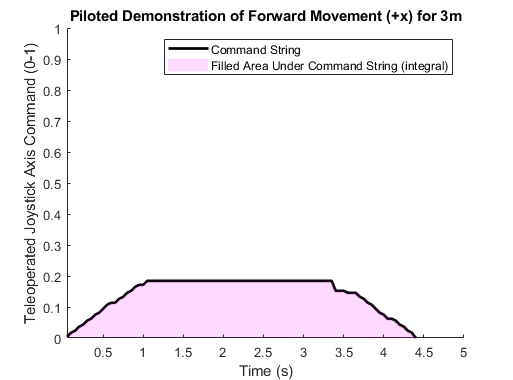
\includegraphics[width=0.48\textwidth]{images/sampleintegral.png}
    \caption{A sample of a single demonstrated flight}
    \label{fig:sampleintegral}
\end{figure}
In Fig. \ref{fig:sampleintegral}, we show a sample of a single flight demonstration. The pilot flies the UAV forward over a distance of approximately $3$ meters. The command string, in this case, corresponds to pitch, where a command of $0$ would imply no pitch adjustment, and $1$ corresponds to the UAV's maximum allowable pitch. The minimum allowable pitch command is $-1$, which would send the UAV in in the negative $y$-direction. Along with the string of commands sent, the shaded portion of Fig.\ref{fig:sampleintegral}, represents the total area under the string of commands, or the integral. Because the pitch is proportional to the linear velocity in the $y$-direction, we theorize that the command string is proportional to the velocity, and its integral, therefore, is proportional to the distance traveled. Lastly, we are interested in the average command sent to the system, as indicated by the dotted line. The integral itself, while conveying information about the distance traveled, lacks precision in that the same integral can be achieved with commands strings of different lengths and heights. Making use of the average command, we are able to improve precision in the process of generating autonomous commands, that must be fixed to a certain length (time) and travel a certain distance.

\section{Methodology}
In our approach, we leverage the data from multiple demonstrations to build a regression model that enables identification of an appropriate integral, $g_u$, and average teleoperation command, $\bar{x}_u$ given a user-set distance, $d_u$, and time, $t_u$. With the appropriate integral and average velocity, the demonstrated command string with the closest integral, $g_i$, to the fitted integral, $g_u$, is resized to match the user-set time, $t_u$ and fitted average velocity, $\bar{x}_u$, to obtain the autonomous command string $\mathbf{x}_a$. This command is sent to the physical UAV for implementation, where the on-board computer collects data regarding the error between actual position, $\mathbf{p}(t)$, and the expected position, $\mathbf{p}_r(t)$ is determined based on the trajectory. This error is reduced by using a proportional controller on the input $\mathbf{x}_a$ to obtain the adjusted input commands, $\mathbf{x}_c$.

    *Block Diagram*

\subsection{Trajectory Generation and Decomposition}
In this section, we examine the target goals and times, $\mathbf{g}$ and $\mathbf{t}$


\subsection{Regression Based Training and Evaluation}
In order to build the appropriate policy for autonomous command generation, we perform offline training on data collected over $m$ human-piloted trials. Because the goal indicated in our problem statement is to be able to track a certain trajectory, the inputs of the training phase are $\{d_i,t_i,\mathbf{x_i}\}$, where $i=1,\ldots,m$, $d_i$ is the distance travelled in each trial, $t_i$ is the length of the trial, and $\mathbf{x_i}$ is the string of teleoperation commands given the by the pilot. In addition to the inputs given by the pilot, we are also interested in two entities \begin{itemize}
    \item The integral of the string of teleoperation commands, $g_i = \int_0^{t_i}\mathbf{x_i}$
    \item The steady-state teleoperation command, $\bar{x}_i \in \mathbf{x_i}$
\end{itemize}
The steady-state command and integral are necessary portions of the analysis because of the directly proportional relationship between teleop commands and system velocity. The steady-state command, in this case, provides information about the pilot's average in-flight velocity, and is obtained by taking the mean of all entries in $\mathbf{x_i}$. The integral, meanwhile, describes the area under the string of commands. Because the teleop commands are proportional to velocity, this area value gives important information about the distance traveled, as position is the integral of velocity over time.

The offline training data is applied to a thin-plate spline surface fit to describe the relationship between training inputs and integral and average velocity. The general form of a thin-plate spline equation is 
\begin{equation}
    f(x,y) = a_1 + a_xx + a_yy + \sum_{i=1}^mw_iU(||(x_i,y_i)-(x,y)||)
\end{equation}

where $a_1,a_x,\text{and}~a_y$ are scalar coefficients, $w_i$ is a coefficient that corresponds to each specific trial, subject to the following condition: \begin{equation}
\sum_{i=1}^mw_i=\sum_{i=1}^mw_ix_i=\sum_{i=1}^mw_iy_i=0
\end{equation}
and the function $U$ is of the form
\begin{equation}
  U(r) = r^2\log{r} 
\end{equation}

Given the corresponding $z_i$ for each $(x_i,y_i)$ pair, we are able to solve the following linear system to obtain the coefficients $w_i,\ldots,w_m$ and $a_1,a_x,a_y$,

\begin{equation}
    \begin{bmatrix}
    K&P\\
    P^T& \mathbf{0}
    \end{bmatrix}
    \begin{bmatrix}
    \mathbf{w}\\
    \mathbf{a}
    \end{bmatrix} = 
    \begin{bmatrix}
    \mathbf{z}\\
    \mathbf{o}
    \end{bmatrix}
\end{equation}

where $K_{ij} = U(||(x_i,y_i)-(x_j,y_j)||)$, $P_i* = (1,x_i,y_i)$, $\mathbf{0}  \in \mathbb{R}^{3\times3}$ is a matrix of zeros, $\mathbf{o} \in \mathbb{R}^{3\times1}$ is a column vector of zeros, $\mathbf{w} \in \mathbb{R}^{m\times1}$ and $\mathbf{z} \in \mathbb{R}^{m\times1}$ are formed from $w_i$ and $z_i$, respectively, and $\mathbf{a}$ is the column vector with elements $a_1,a_x,a_y$.

Given the general framework for performing the thin-plate spline, we develop two separate relationships for our specific application: $g_i = f(d_i,t_i)$ and $\bar{x}_i = h(d_i,t_i)$
With the functions we have obtained, we are able to find an estimated integral and steady-state command, $g_u$ and $\bar{x}_u$, for any given desired distance and time,

\begin{equation} \label{eq:integralfit}
g_u = f(d_u,t_u)
\end{equation}
\begin{equation} \label{eq:ssvelfit}
\bar{x}_u = h(d_u,t_u)
\end{equation}

where $d_u$ and $t_u$ are the user-set desired distance and time, respectively.

While a thin-plate spline is continuous, and a result can be obtained with any combination of distance and time as an input pair, the accuracy of the results of any pair $(d_u,t_u)$ can suffer as the distance between evaluation points and training points increases [CITE]. In order to quantify this, we leverage the standard error of the estimate, which is a statistic used to measure the accuracy of predictions given a certain type of regression with known values:
\begin{equation} \label{eq:stderr}
    \sigma_{est} \approx \frac{s}{\sqrt{m}}
\end{equation}
where $s$ is the sample standard deviation of all of the points in the training set and $m$ is the number of training samples. The standard error, $\sigma_{est}$, is then used to determine the t-statistic for different test values. The t-statistic is defined as the ratio of departure of a test point from a known point to its standard error and is defined as
\begin{equation} \label{eq:tstat}
t_{\hat{\beta}} = \frac{|\hat{\beta}-\bar{\beta}|}{\sigma_{est}}    
\end{equation}
where $\hat{\beta}$ is the test point and $\bar{\beta}$ is the nearest known point. In equation \eqref{eq:tstat}, if $t_{\hat{\beta}} \geq 1$, that means that the test point $\hat{\beta}$ propagates an error higher than the standard error. As a result, it is desirable to have $t_{\hat{\beta}} < 1$. Using a certain set-point for the t-statistic, the maximum allowable departure from known points is obtained:
\begin{equation}
    \sigma_{est}t_{\hat{\beta}} = |\hat{\beta}-\bar{\beta}|
\end{equation}
The appropriate departure is used to set the bounds for each training data point, for example:
\begin{align}
    \hat{\beta}_{\min} = \bar{\beta} - \sigma_{est}t_{\hat{\beta}} \nonumber \\
    \hat{\beta}_{\max} = \bar{\beta} + \sigma_{est}t_{\hat{\beta}}
\end{align}
where $\beta_{\min}$ and $\beta_{\max}$ are the lower and upper bounds for known parameter $\bar{\beta}$.

In our case, there are two parameters we are primarily concerned about for prediction; distance and time. As a result, we perform this calculation twice over, treating each of the two parameters as statistically independent, to obtain a generic interval for each point in the training set, denoted $[d_{i\min},d_{i\max}]$ and $[t_{i\min},t_{i\max}]$, where $i=1,\ldots,m$. Because we are ultimately interested in using the distance and time values together as input pairs, we then obtain a maximum Euclidean distance from each of the training data points using:

\begin{equation}
    \Delta_i = \sqrt{(\sigma_{d_{est}})^2+(\sigma_{t_{est}})^2}
\end{equation}
Using the maximum distance for each point $\Delta_i$, we are able the generate intervals around each point, where the data is within the standard error of the estimate.


\subsection{Autonomous Behaviour Generation}

In order for the system to autonomously reach a user-set goal, $g_u$ and $\bar{x}_u$ are obtained using equations \eqref{eq:integralfit} and \eqref{eq:ssvelfit}, and the offline training samples are leveraged to generate a new string of commands.

From the training set of $m$ samples, we select the trial that has the closest integral, $g_i$, to the estimated integral $g_u$. This is done by forming an error vector, $\mathbf{e}\in\R^{1\times m}$, where each element is defined by
\begin{equation}
 e_i = \vert g_i-g_u \vert , ~i= \{1,\ldots,m\}
\end{equation}
 The lowest error is then found and is paired with the appropriate pre-trained sample, $\mathbf{x}^*$,

\begin{equation}
\mathbf{x}^* = \mathbf{x}_i \in \mathbf{x}\vert e_i = \min_e(\mathbf{e})
\end{equation}

This optimal pre-trained sample is then adjusted to reflect the user-set time, $t_u$. This is done by performing bicubic interpolation to re-size the vector $\mathbf{x}^*$. Interpolation methods to re-size vectors are used so that important information is not lost and features are kept the same. This method is often used for re-sizing complex images, and has shown effectiveness in . Bicubic interpolation is the chosen method for re-sizing, as it performs better than nearest-neighbor and bilinear interpolation methods, while only marginally increasing computational complexity. The general form of a bicubic interpolation equation is 

\begin{equation}
    p(x) = \sum_{i=0}^3a_ix^i
\end{equation}

where $x$ is an entry in vector $\mathbf{x}^*$ and $a$ represents the coefficients of the function at each point. Bicubic interpolation takes the weighted sum of the four nearest neighbors of each entry in the command vector in order to identify the intermediate points between each value in $\mathbf{x}^*$. After resizing, we obtain the time adjusted input vector $\mathbf{x}'$. The time-adjusted command vector is obtained in this manner 

The next step is to adjust the input vector such that the system reaches the user-set goal $d_u$. This is done by leveraging the average velocity information, that is, $\bar{x}_u$. Because distance is a function of average velocity and time, the scale time-adjusted vector $\mathbf{x}'$ is scaled such that its mean is equivalent to $\bar{x}_u$. We then obtain
\begin{equation}
\mathbf{x}_a = \mathbf{x}'\bigg(\frac{\bar{x}_u}{\bar{x}'}\bigg)
\end{equation}

The input $\mathbf{x}_a$ is then sent to the UAV to reach the goals set by the users. In Fig.\ref{fig:gensample}, we show visually the steps of command generation. In Fig.\ref{fig:ogstring}, we start with the original pre-trained command string that was shown above in Fig.\ref{fig:sampleintegral}. This flight travelled approximately $4.4$ seconds for $3$ meters. For testing purposes, our use input values are $d_u=3.5$m and $t_u=3.75$s. As indicated, a time adjustment is made first; this is shown in Fig.\ref{fig:timeadj}. It is important to note that the average command, indicated by the dashed line, is still the same. 


\begin{figure}[h]
	\centering
	\subfigure[Original String \label{fig:ogstring}]{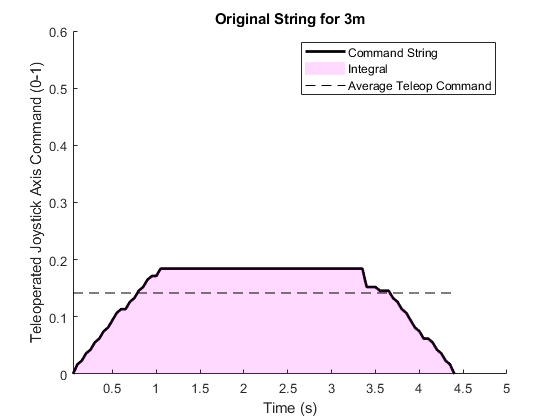
\includegraphics[width=0.3\linewidth]{images/ogstring.png}}
	\subfigure[Time Adjustment \label{fig:timeadj}]{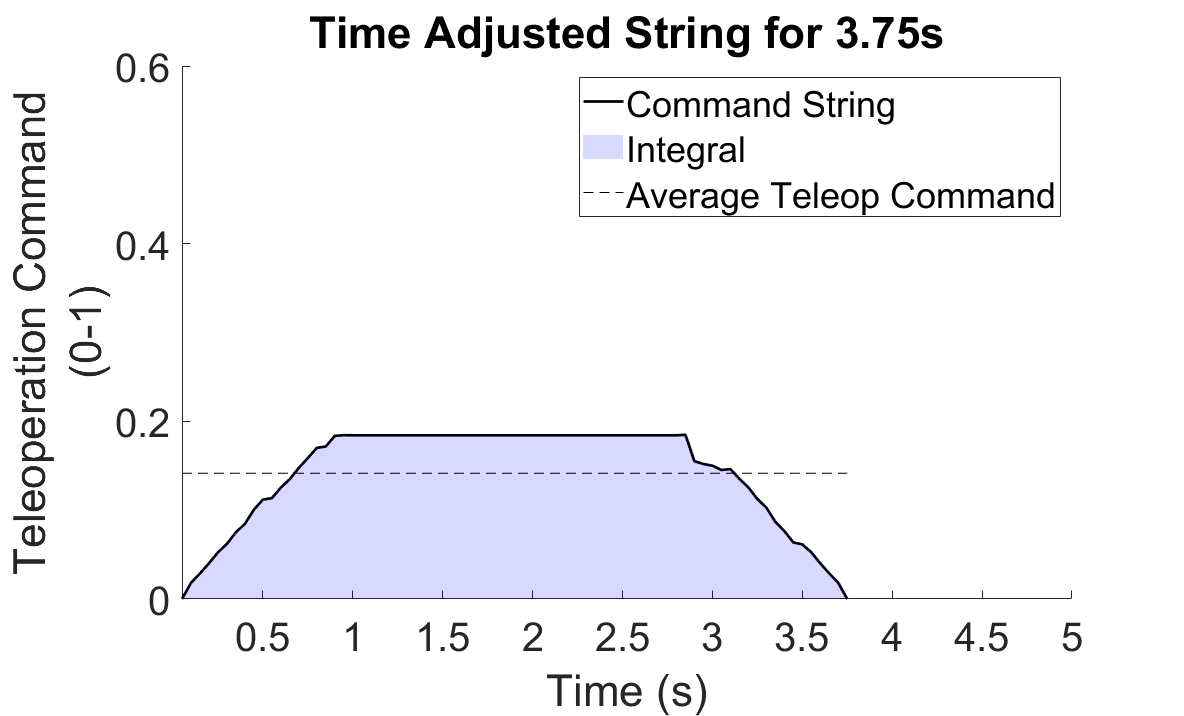
\includegraphics[width=0.3\linewidth]{images/timeadj.png}}
    \subfigure[Final Commands \label{fig:fullyadj}]{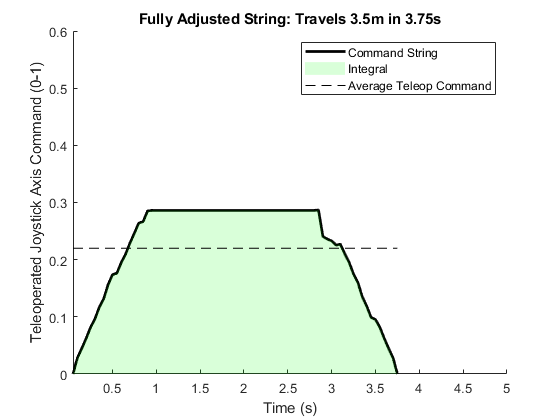
\includegraphics[width=0.3\linewidth]{images/fullyadj.png}}
	\caption{Command Generation Process}
	\label{fig:gensample}
	\vspace{-15pt}
\end{figure}

\subsection{Online Adaptation of Generated Commands}

The commands generated in the previous section are generated and sent to the UAV in open-loop. In order to close the loop, we propose a method to control for any possible error. While executing generated command string, $\mathbf{x_a}(t)$, we constantly monitor for error between the position of the vehicle, $\mathbf{p}(t)$ and the reference position as per the generated trajectory, $\mathbf{p_r}(t)$:

\begin{equation}
    \xi(t) = \mathbf{p}(t)-\mathbf{p_r}(t)
\end{equation}

The error $\xi(t)$ is attributed to the most recent command $\mathbf{x}_a(t)$, and a proportional controller is used to adjust the following command $\mathbf{x}_a(t+1)$ to obtain the closed-loop command $\mathbf{x}_c(t+1)$ as follows

\begin{equation}
    \mathbf{x}_c(t+1) = \mathbf{x}_a(t+1) + k_p(t)\xi(t)
\end{equation}

The proportional gain, $k_p(t)$, is automatically tuned based loosely off the Ziegler-Nichols method [CITE] where the proportional gain is increased until there is stable and consistent oscillation in the output, which in our case, is the position error, $\xi(t)$. In order to set the interval of gain increase each iteration, we leverage the ratio of reference position to actual position:
\begin{equation}
    k_p(t+1) = k_p(t) + \bigg(\frac{\mathbf{p_r}(t)}{\mathbf{p}(t)}\bigg)\bigg(\frac{1}{t_u}\bigg)
\end{equation}
where $t_u$ refers to the user-set time, and adjusts the update of $k_p$ such that the rate of increase is controlled for iteration time. Not adjusting in this manner would suggest that the controller is controlling for error over the entire remaining string of commands, rather than the first subsequent command.






\section{Experiments}


\section{Conclusions}

\section{Acknowledgement}


\addtolength{\textheight}{-12cm}   % This command serves to balance the column lengths
                                  % on the last page of the document manually. It shortens
                                  % the textheight of the last page by a suitable amount.
                                  % This command does not take effect until the next page
                                  % so it should come on the page before the last. Make
                                  % sure that you do not shorten the textheight too much.

%%%%%%%%%%%%%%%%%%%%%%%%%%%%%%%%%%%%%%%%%%%%%%%%%%%%%%%%%%%%%%%%%%%%%%%%%%%%%%%%

%References are important to the reader; therefore, each citation must be complete and correct. If at all possible, references should be commonly available publications.



\begin{thebibliography}{99}

\bibitem{c1} G. O. Young, �Synthetic structure of industrial plastics (Book style with paper title and editor),� 	in Plastics, 2nd ed. vol. 3, J. Peters, Ed.  New York: McGraw-Hill, 1964, pp. 15�64.
\bibitem{c2} W.-K. Chen, Linear Networks and Systems (Book style).	Belmont, CA: Wadsworth, 1993, pp. 123�135.
\bibitem{c3} H. Poor, An Introduction to Signal Detection and Estimation.   New York: Springer-Verlag, 1985, ch. 4.


\end{thebibliography}




\end{document}
